\documentclass[12pt,openright]{report}
\pagestyle{headings}
\usepackage{layout} 
\usepackage[left=1.4in, right=1.0in, top=1.2in, bottom=1.2in]{geometry} %page margin


\usepackage[utf8]{inputenc}
%\usepackage[brazil]{babel}
%\usepackage{biblatex} %Bibliografia. Cita sites
\usepackage{url}
%%%%%%%%%%%%%%%%%%%%%%%%
%\usepackage[latin1]{inputenc} -> separação de silabas


%\usepackage{pslatex} %Times New Roman Font 
\usepackage{fontenc}
\usepackage{verbatim} %inclui comentários em blocos
\usepackage{indentfirst} %primeiro paragrado identado

%%%%%%%%%%%%%%%%%%%% simbolos matematicos
\usepackage[intlimits]{amsmath} %limites do lim ficam embaixo!
\usepackage{amsthm, amssymb} 
%%%%%%%%%%%%%%%%%%%

%%%%%%%%%%%%%%%%%%%% fontes matematicas
\usepackage{amsfonts, mathrsfs} 
%\usepackage{bbold} % modifica o \mathbb para fazer matriz identidade
%%%%%%%%%%%%%%%%%%%


\usepackage{graphicx,color,array}
\usepackage{float} %para usar comando [H] na fig e posicionar figuras onde quero
%\usepackage{mathtools} %inclui automaticamente o 'amsmath'
\usepackage{multicol}

%\usepackage{mathtools} %inclui automaticamente o 'amsmath'

\usepackage{ctable}

%\usepackage{natbib} % bibliography style file

%%%%%%%%%%%%%%%%%%%% esteticos
\setlength{\belowcaptionskip}{10pt} %espaço abaixo do caption
%%%%%%%%%%%%%%%%%%%


\usepackage[portuguese,ruled,vlined,linesnumbered,boxed]{algorithm2e} % Pacote para escrever algoritmos em Portugol
\renewcommand{\algorithmautorefname}{Algoritmo}% para utilizar \autoref

% Adicione o trecho a seguir somente se desejar incluir uma Lista de algoritmos (opcional)
%\renewcommand{\listalgorithmcfname}{Lista de algoritmos}%
%\renewcommand{\listasdousuario}{
%  \pdfbookmark[0]{\listalgorithmcfname}{loa}
%  \listofalgorithms
%  \cleardoublepage
%}




%%%%%%%%%%%%%%%%%%% não estão sendo usados!
%\usepackage{tikz}      %gera fluxograma
%\usetikzlibrary{shapes,arrows}
%\usepackage{placeins} %permite fixar barreiras para posicionar as fig

%%%%%%%%%%%%%%%%%%% modifica simbolos do footnote!
%1 - *
%2 - dagger
%3 - double dagger
%4 - ... 9 (see page 175 of the latex manual)
%\long\def\symbolfootnote[#1]#2{\begingroup%
%\def\thefootnote{\fnsymbol{footnote}}\footnote[#1]{#2}\endgroup}
%%%%%%%%%%%%%%%%%%%

%%%%%%%%%%%%%%%%%%%% new command
\newcommand{\blue}[1]{\textcolor{blue}{#1}\index{#1@\textcolor{blue}{#1}}}

\newcommand{\be}{\begin{equation}}
\newcommand{\ee}{\end{equation}}
\newcommand{\benn}{\begin{equation*}}
\newcommand{\eenn}{\end{equation*}}
\newcommand{\bi}{\begin{itemize}}
\newcommand{\ei}{\end{itemize}}
\newcommand{\bdm}{\begin{displaymath}}
\newcommand{\edm}{\end{displaymath}}
\newcommand{\half}{\frac{1}{2}}
\newcommand{\nn}{\nonumber \\}

%\def\citeapos#1{\citeauthor{#1}'s (\citeyear{#1})} %install te.bst style

%\def\reindex #1 #2\sentinel{\index{#2, #1}}
%\newcommand{\person}[1]{#1\reindex #1\sentinel}


%%%%%%%%%%%%%%%%%%%%%%%%%%%%%%%%%%%%%%%%%%%%%

\title{\bf {Relatório}}
\author{Karine Piacentini Coelho da Costa\footnote{karinepcdc@ufrn.br}}%


%%%%%%%%%%%%%%%%%%%%%%%%%%%%%%%%%%%%%%%%%%%%%%%%%
%%%%%%%%%%%%%% DOCUMENT BODY %%%%%%%%%%%%%%%%%%%%
%%%%%%%%%%%%%%%%%%%%%%%%%%%%%%%%%%%%%%%%%%%%%%%%%
\begin{document}

%%%%%%% FRONT MATTERS %%%%%%%%%%%
%\input{Front.tex}
\maketitle

%\newpage
%\thispagestyle{empty}
%\mbox{}

\newpage
\pagenumbering{arabic}
\tableofcontents

\newpage
%\input{1_sumReport.tex}

\newpage

%\newpage
%\thispagestyle{empty}
%\mbox{}
%\newpage

%%%%%%% MAIN MATTERS %%%%%%%%%%%%
\chapter{Introdução}

Esse relatório descreve uma análise de complexidade empírica de diferentes algoritmos de busca. São considerados os seguintes algoritmos de busca: busca linear; busca binária (versões iterativas e recursiva); busca ternária (versões iterativas e recursiva); {\it jump search}; e busca de Fibonacci.

O primeiro objetivo desse estudo é determinar qual dos dois algoritmos lineares são mais eficientes (a busca linear ou a {\it jump search}). O segundo objetivo é determinar qual implementação é mais eficiente, a recursiva ou iterativa. O terceiro, é determinar como o tamanho da partição influência nos algoritmos de busca não lineares. O quarto é determinar a partir de que momento algoritmos de classe de complexidade diferentes se diferenciam (comparando a busca linear com a binária). Por fim, o quinto objetivo procura determinar se existe diferentes categorias de cenários pior caso para o algoritmo de busca de Fibonacci.

\chapter{Metodologia}

Nesta seção descrevemos os materiais e a metodologia utilizados para obteção dos resultados apresentados no capítulo 3.

\section{Características técnicas}

Os algorítmos de buscas foram implementados na linguagem C++ e o compilador utilizado foi o g++ (tipo e versão????). O computador onde as simulações foram realizadas possui as seguintes características:
\begin{itemize}
\item[-] MacBook Pro (2014)
\item[-] Processador: 2.5 Ghz Intel Core i7
\item[-] memória: 16 GB 1600 MHz DDR3
\item[-] Placa mãe: ????
\item[-] Sistema operaciona: (tipo e versão????)
\end{itemize}

\section{Algoritmos}

Os algoritmos de busca utilizados nesse estudo estão apresentados aqui com uma breve descrição. Os códigos utilizados encontram-se no apêndice 1. ????


%%%%%%%%%%%%%%%%%%%%%%%%%
%%% Algorithm2e codes %%%

\SetKwProg{Fnc}{Função}{}{fim}
\SetKwFunction{buscaLin}{buscaLin}
\SetKwFunction{buscaBin}{buscaBin\_it}
\SetKwFunction{buscaBinrec}{buscaBin\_rec}
\SetKwFunction{buscaTer}{buscaTer\_it}
\SetKwFunction{buscaTerrec}{buscaTer\_rec}
\SetKwFunction{buscaJump}{buscaJump}
\SetKwFunction{buscaFib}{buscaFib}
\SetKw{Ate}{até}
\SetKw{E}{e}
\SetKwArray{vet}{V}
%%%%%%%%%%%%%%%%%%%%%%%%%
\subsection{Busca linear}


\begin{algorithm}[H]
  \DontPrintSemicolon
  \SetAlgoLined
  \caption{Busca linear}

  \Entrada{Vetor $V$, chave $k$ e limites de busca esquerdo $l$ e direito $r$ (inclusive).}
  \Saida{Índice da ocorrência de $k$ em $V$; ou $-1$ caso não exista $k$ em $V$.}
  \tcc{Precondição: $l \leq r$; $l,r \geq 0$; $V$ em ordem crescente.}  
  \BlankLine

  \Fnc{\buscaLin{$V$: {\bf arranjo de inteiros}; $l$: {\bf inteiro}; $r$: {\bf inteiro}; $k$: {\bf inteiro}}: {\bf inteiro}}{
    {\bf var} $i$: {\bf inteiro} \;
    \Para{$i \leftarrow l \; \Ate \; r$}{
      \Se{$\vet{i} \; == \; k$}{
        \Retorna{$i$}
      }       
    }

    \Retorna{$-1$}
  }
\end{algorithm}



\subsection{Busca binária}

\begin{algorithm}[H]
  \DontPrintSemicolon
  \SetAlgoLined
  \caption{Busca binária iterativa}

  \Entrada{Vetor $V$, chave $k$ e limites de busca esquerdo $l$ e direito $r$ (inclusive).}
  \Saida{Índice da ocorrência de $k$ em $V$; ou $-1$ caso não exista $k$ em $V$.}
  \tcc{Precondição: $l \leq r$; $l,r \geq 0$; $V$ em ordem crescente.}  
  \BlankLine

  \Fnc{\buscaBin{$V$: {\bf arranjo de inteiros}; $l$: {\bf inteiro}; $r$: {\bf inteiro}; $k$: {\bf inteiro}}: {\bf inteiro}}{
    {\bf var} $m$: {\bf inteiro} \tcc{último valor da primeira metade do arranjo} \;
    \Enqto{$r \geq \;l$}{
      $m \leftarrow (l+r)/2$\;
      \uSe{$k \; == \; \vet{m}$}{
        \Retorna{$m$}
      } \uSenaoSe{$k \; < \; \vet{m}$}{
        $r \leftarrow m-1$\;
      } \Senao{
        $l \leftarrow m+1$\;
      }
      
    }

    \Retorna{$-1$}
  }
\end{algorithm}


\begin{algorithm}[H]
  \DontPrintSemicolon
  \SetAlgoLined
  \caption{Busca binária recursiva}

  \Entrada{Vetor $V$, chave $k$ e limites de busca esquerdo $l$ e direito $r$ (inclusive).}
  \Saida{Índice da ocorrência de $k$ em $V$; ou $-1$ caso não exista $k$ em $V$.}
  \tcc{Precondição: $l \leq r$; $l,r \geq 0$; $V$ em ordem crescente.}  
  \BlankLine
  
  \Fnc{\buscaBinrec{$V$: {\bf arranjo de inteiros}; $l$: {\bf inteiro}; $r$: {\bf inteiro}; $k$: {\bf inteiro}}: {\bf inteiro}}{
    {\bf var} $m$: {\bf inteiro} \tcc{último valor da primeira metade do arranjo} \;
    \uSe{$r < \;l$}{
      \Retorna{$-1$}
    } \Senao{

      $m \leftarrow (l+r)/2$\;
      \uSe{$k \; == \; \vet{m}$}{
        \Retorna{$m$}
      } \uSenaoSe{$k \; < \; \vet{m}$}{
        \Retorna \buscaBinrec{$V$,$l$,$m-1$,$k$}\;
      } \Senao{
        \Retorna \buscaBinrec{$V$,$m+1$,$r$,$k$}\;
      }
      
    }

  }
\end{algorithm}



\subsection{Busca ternária}

\begin{algorithm}[H]
  \DontPrintSemicolon
  \SetAlgoLined
  \caption{Busca ternária iterativa}

  \Entrada{Vetor $V$, chave $k$ e limites de busca esquerdo $l$ e direito $r$ (inclusive).}
  \Saida{Índice da ocorrência de $k$ em $V$; ou $-1$ caso não exista $k$ em $V$.}
  \tcc{Precondição: $l \leq r$; $l,r \geq 0$; $V$ em ordem crescente.}  
  \BlankLine

  \Fnc{\buscaTer{$V$: {\bf arranjo de inteiros}; $l$: {\bf inteiro}; $r$: {\bf inteiro}; $k$: {\bf inteiro}}: {\bf inteiro}}{
    {\bf var} $t_{1}$: {\bf inteiro} \tcc{último valor do primeiro terço do arranjo}
    {\bf var} $t_{2}$: {\bf inteiro} \tcc{último valor do segundo terço do arranjo} \;
    \Enqto{$r \geq \;l$}{
      $t_{1} \leftarrow l+(r-l)/3$\;
      $t_{2} \leftarrow r-(r-l)/3$\;\;
      \uSe{$k \; == \; \vet{$t_{1}$}$}{
        \Retorna{$t_{1}$}
      } \uSenaoSe{$k \; == \; \vet{$t_{2}$}$}{
        \Retorna{$t_{2}$}
      } \uSenaoSe{$k \; < \; \vet{$t_{1}$}$}{
        $r \leftarrow t_{1}-1$\;
      } \uSenaoSe{$k \; < \; \vet{$t_{2}$}$}{
        $l \leftarrow t_{1}+1$\;
        $r \leftarrow t_{2}-1$\;
      } \Senao{
        $l \leftarrow t_{2}+1$\;
      }
      
    }

    \Retorna{$-1$}
  }
\end{algorithm}


\begin{algorithm}[H]
  \DontPrintSemicolon
  \SetAlgoLined
  \caption{Busca ternária recursiva}

  \Entrada{Vetor $V$, chave $k$ e limites de busca esquerdo $l$ e direito $r$ (inclusive).}
  \Saida{Índice da ocorrência de $k$ em $V$; ou $-1$ caso não exista $k$ em $V$.}
  \tcc{Precondição: $l \leq r$; $l,r \geq 0$; $V$ em ordem crescente.}  
  \BlankLine
  
  \Fnc{\buscaTerrec{$V$: {\bf arranjo de inteiros}; $l$: {\bf inteiro}; $r$: {\bf inteiro}; $k$: {\bf inteiro}}: {\bf inteiro}}{
    {\bf var} $t_{1}$: {\bf inteiro} \tcc{último valor do primeiro terço do arranjo}
    {\bf var} $t_{2}$: {\bf inteiro} \tcc{último valor do segundo terço do arranjo} \;    
    \uSe{$r < \;l$}{
      \Retorna{$-1$}
    } \Senao{
      $t_{1} \leftarrow l+(r-l)/3$\;
      $t_{2} \leftarrow r-(r-l)/3$\;\;
      \uSe{$k \; == \; \vet{$t_{1}$}$}{
        \Retorna{$t_{1}$}
      } \uSenaoSe{$k \; == \; \vet{$t_{2}$}$}{
        \Retorna{$t_{2}$}
      } \uSenaoSe{$k \; < \; \vet{$t_{1}$}$}{
        \Retorna \buscaTerrec{$V$,$l$,$t_{1}-1$,$k$}
      } \uSenaoSe{$k \; < \; \vet{$t_{2}$}$}{
        \Retorna \buscaTerrec{$V$,$t_{1}+1$,$t_{2}-1$,$k$}
      } \Senao{
        \Retorna \buscaTerrec{$V$,$t_{2}+1$,$r$,$k$}
      }
      
    }

  }
\end{algorithm}


\subsection{{\it Jump search}}

\begin{algorithm}[H]
  \DontPrintSemicolon
  \SetAlgoLined
  \caption{{\it Jump search}}

  \Entrada{Vetor $\vet$, chave $k$ e limites de busca esquerdo $l$ e direito $r$ (inclusive).}
  \Saida{Índice da ocorrência de $k$ em $V$; ou $-1$ caso não exista $k$ em $V$.}
  \tcc{Precondição: $l \leq r$; $l,r \geq 0$; $V$ em ordem crescente.}  
  \BlankLine

  \Fnc{\buscaJump{$V$: {\bf arranjo de inteiros}; $l$: {\bf inteiro}; $r$: {\bf inteiro}; $k$: {\bf inteiro}}: {\bf inteiro}}{
    {\bf var} $m$: {\bf inteiro} \;
    {\bf var} $p$: {\bf inteiro} \tcc{tamanho do salto}\;

    $p \leftarrow \sqrt{r-l+1}$\;
    $m \leftarrow l+p$\;
    
    \Enqto{$m \leq r$}{
      \uSe{$k \; == \; \vet{m}$}{
        \Retorna $m$\;
      }\SenaoSe{$k \; < \;\vet{m}$}{
        \Retorna{\buscaLin{$\vet,m-p,m-1,k$}}
      }
      $m \leftarrow m + p$
    }

    \Se{$m>r$ \E $\vet{r} > k$}{
      \Retorna{\buscaLin{$\vet,m-p,r,k$}}
    }

    \Retorna{$-1$}
  }
\end{algorithm}



\subsection{Busca de Fibonacci}


\begin{algorithm}[H]
  \DontPrintSemicolon
  \SetAlgoLined
  \caption{Busca de Fibonacci}
  \Entrada{Vetor $V$, chave $k$ e limites de busca esquerdo $l$ e direito $r$ (inclusive).}
  \Saida{Índice da ocorrência de $k$ em $V$; ou $-1$ caso não exista $k$ em $V$.}
  \tcc{Precondição: $l \leq r$; $l,r \geq 0$; $V$ em ordem crescente.}  
  \BlankLine

  \Fnc{\buscaBin{$V$: {\bf arranjo de inteiros}; $l$: {\bf inteiro}; $r$: {\bf inteiro}; $k$: {\bf inteiro}}: {\bf inteiro}}{
    {\bf var} $size$: {\bf inteiro}\;
    {\bf var} $i$: {\bf inteiro}\;
    {\bf var} $i_{fib1}$: {\bf inteiro}\;
    {\bf var} $fib1$: {\bf inteiro}\;
    {\bf var} $Fib$: {\bf arranjo de inteiros}\;

    $size \leftarrow r-l+1$\;

    \tcc{Calcula a serie de Fibonacci até o i-ésimo termo,\; onde F(i) <= size}
    $Fib[0] \leftarrow 0$\;
    $Fib[1] \leftarrow 1$\;

    $i \leftarrow 1$\;
    \Enqto{ $Fib[i] < size$}{
      $i \leftarrow i + 1$\;
      $Fib[i] \leftarrow Fib[i-1] + Fib[i-2]$\;
    }\;
    
    $i_{fib1} \leftarrow i-2$\;
    \Enqto{$l<r$}{
      
      $fib1 \leftarrow l + F[i_{fib1}]$\;
      \uSe{$k == V[fib1]$}{
        \Retorna $fib1$\;
      } \uSenaoSe{$k < V[fib1]$}{ \tcc{Novos tamanhos das partições à esquerda}
        $r\leftarrow i_{fib1}-1$\;
        $i_{fib1} = i_{fib1}-2$\;
        \Se{$i_{fib1}<0$}{
          $i_{fib1}\leftarrow 0$\;
        }
      } \Senao{ \tcc{Procure os novos tamanhos das partições à direita}
        $l\leftarrow i_{fib1}+1$\;
        $i \leftarrow  \; i_{fib1}+1$\;
        \Enqto{$Fib[i] < r-l+1$}{
            $i \leftarrow i - 1$\;
        }
        $i_{fib1} = i-1$\;
        }
        
      }  
      
    
    \Retorna{$-1$}
  }
\end{algorithm}


\section{Cenários das simulações}

As simulações foram feitas buscando um valor em um conjunto {\it ordenado crescente}. Consideramos o pior caso apenas, ou seja a busca de um valor que não pertence ao conjunto de busca, mas que é maior que o maior elemento neste conjunto.

\section{metodologia}
%% descrição do método ou procedimento empregado para gerar os dados do experimento, quais e como as medições foram tomadas para comparar os algoritmo (tempos, passos, memória)...

Um vetor de inteiros longos de tamanho $10^8$ preenchido com números pares em ordem crescente foi utilizado para gerar as amostras.

Amostras de arranjo

\subsection{Simulações de tempo de execução}

média temporal progressiva...

\subsection{Simulações do número de passos da operação dominante}

\chapter{Resultados}

Os resultados obtidos com as simulações estão descrito abaixo.

\section{Busca linear}

Na figura abaixo temos o resultado de .... Fazendo um ajuste dos pontos da curva conseguimos determinar que o comportamento é linear.


\begin{figure}[H]
  \centering
  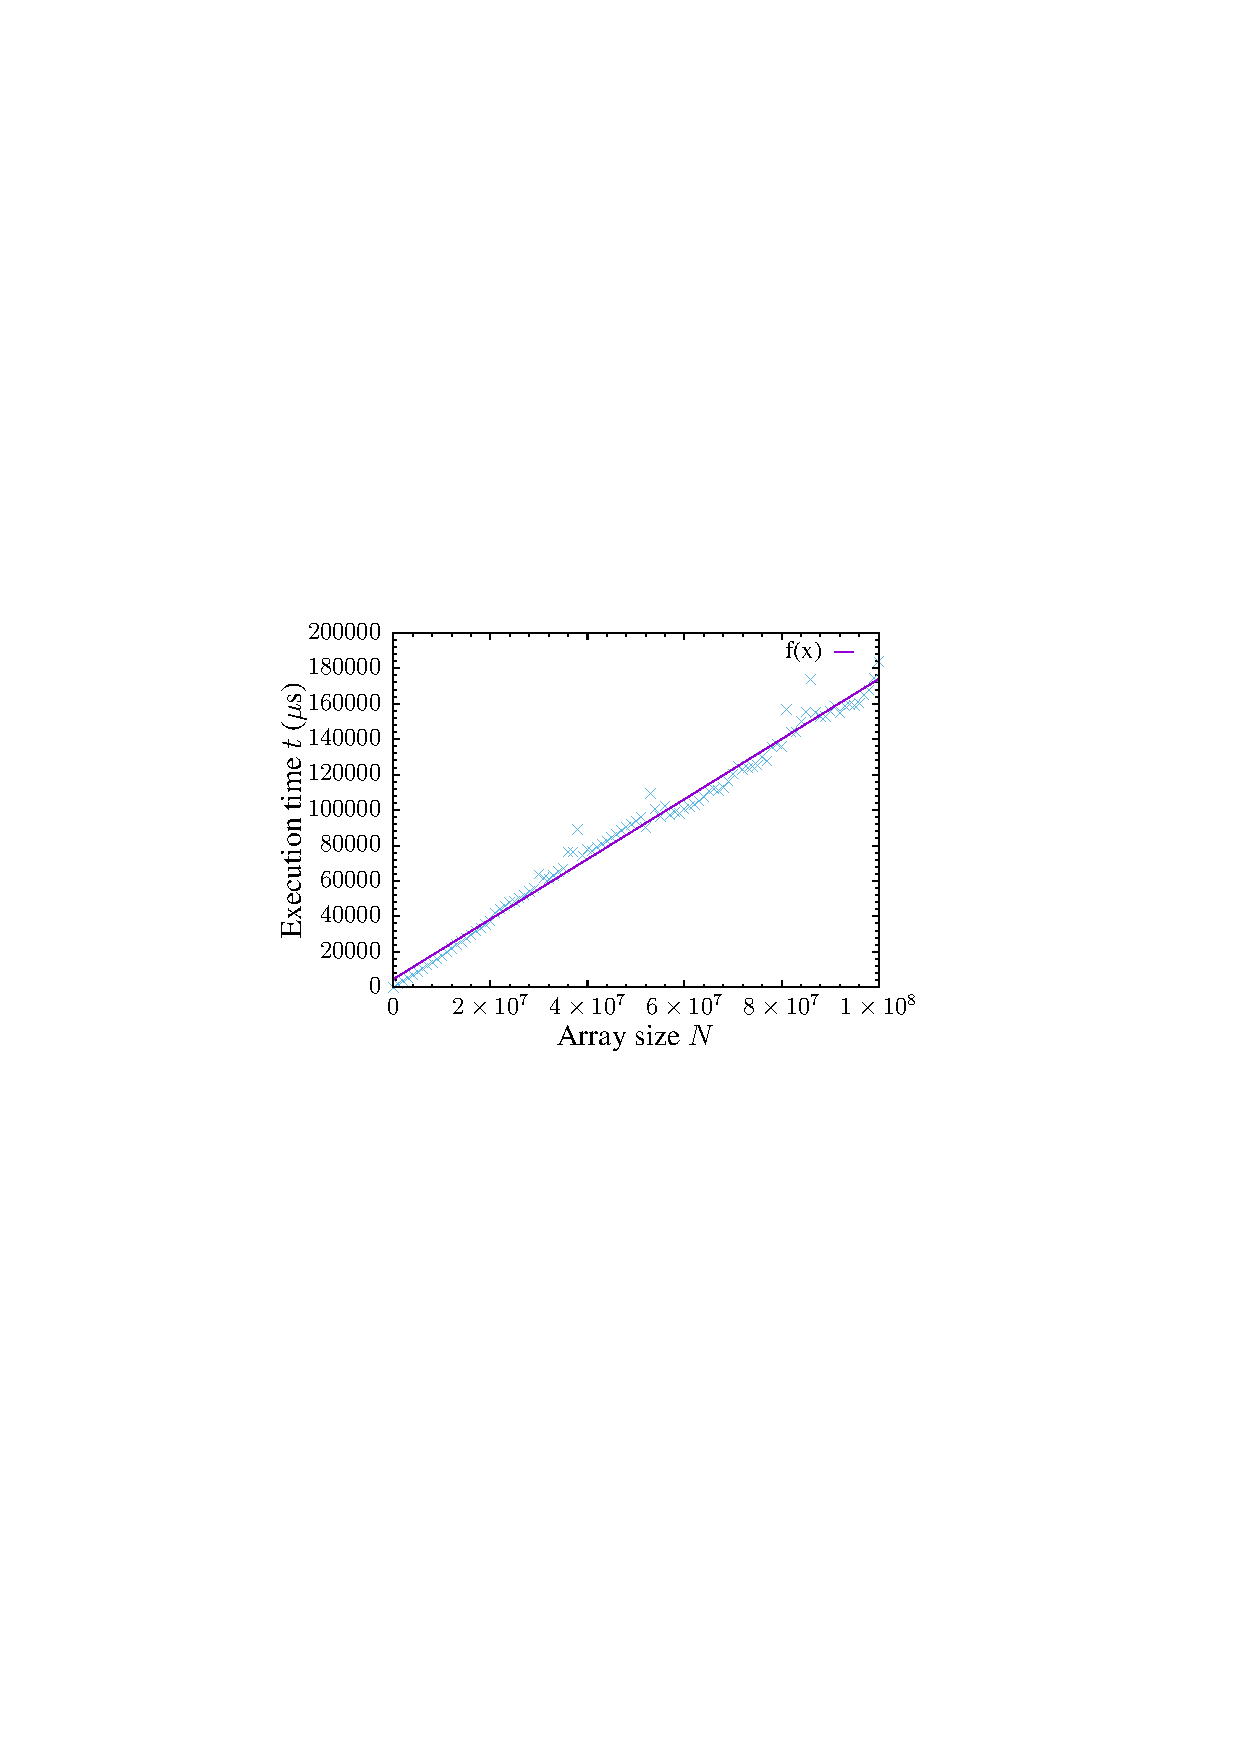
\includegraphics[scale=1.2]{../plots/lsearch_time.pdf}
  \caption{Tempo vs...}
\end{figure} \label{fig:lseach_time}


\section{Busca binária}

Na figura abaixo temos o resultado de .... Fazendo um ajuste dos pontos da curva conseguimos determinar que o comportamento é logarítmico.


\begin{figure}[H]
  \centering
  \includegraphics[scale=1.2]{../plots/bsearch_it_time.pdf}
  \caption{Tempo vs...}
\end{figure} \label{fig:bseach_it_time}

Na figura abaixo temos o resultado de .... Fazendo um ajuste dos pontos da curva conseguimos determinar que o comportamento é logarítmico.


\begin{figure}[H]
  \centering
  \includegraphics[scale=1.2]{../plots/bsearch_rec_time.pdf}
  \caption{Tempo vs...}
\end{figure} \label{fig:bseach_rec_time}


\section{Busca ternária}

Na figura abaixo temos o resultado de .... Fazendo um ajuste dos pontos da curva conseguimos determinar que o comportamento é logarítmico.


\begin{figure}[H]
  \centering
  \includegraphics[scale=1.2]{../plots/tsearch_it_time.pdf}
  \caption{Tempo vs...}
\end{figure} \label{fig:tseach_it_time}

Na figura abaixo temos o resultado de .... Fazendo um ajuste dos pontos da curva conseguimos determinar que o comportamento é logarítmico.


\begin{figure}[H]
  \centering
  \includegraphics[scale=1.2]{../plots/tsearch_rec_time.pdf}
  \caption{Tempo vs...}
\end{figure} \label{fig:tseach_rec_time}

\section{{\it Jump search}}

Na figura abaixo temos o resultado de .... Fazendo um ajuste dos pontos da curva conseguimos determinar que o comportamento se aproxima de um comportamento quadrático.


\begin{figure}[H]
  \centering
  \includegraphics[scale=1.2]{../plots/jumpsearch_time.pdf}
  \caption{Tempo vs...}
\end{figure} \label{fig:jumpsearch_time}

\section{Busca de Fibonacci}

pc\chapter{Discussão}

Nesta seção, são analidos os resultados obtidos a fim de responder as perguntas que motivaram este estudo.

\section{Algoritmos linear mais eficiente}

A primeira pergunta a ser respondida é qual dos dois algoritmos lineares simulados é mais eficiente. Na figura \ref{fig:lvsj_search_time}, estão os resultados da busca linear e da {\it jump search}. Claramente, a {\it jump search} é mais eficiente, chegando a ser mil vezes mais rápida para o maior tamanho de arranjo simulado. Na ampliação mostrada na figura \ref{fig:lvsj_search_time_zoom} podemos observar melhor a diferença de eficiência entre os dois algoritmos. 

\begin{figure}[H]
  \centering
  \includegraphics[scale=1.2]{../plots/lvsj_search_time.pdf}
  \caption{Comparação do tempo de execução médio das simuluções dos algoritmos lineares: busca linear (preto) e {\it jump search} (verde).}
  \label{fig:lvsj_search_time}
\end{figure} 

\begin{figure}[H]
  \centering
  \includegraphics[scale=1.2]{../plots/lvsj_search_time_zoom.pdf}
  \caption{Ampliação da figura \ref{fig:lvsj_search_time}.}
  \label{fig:lvsj_search_time_zoom}
\end{figure} 


\section{Implementação mais eficiente: recursiva ou iterativa?}

O segundo objetivo é determinar qual implementação é mais eficiente, se a recursiva ou a iterativa. Analisando as curvas mostradas nas figuras \ref{fig:bsearch_ivsr_time} e \ref{fig:tsearch_ivsr_time} verifica-se que a versão iterativa e recursiva se diferenciam muito pouco, tanto na versão binária ou ternária do algoritmo. Para alguns tamanhos a curva da implementação iterativa parece ligeiramente mais eficiente, no entanto a medida de tempo de execução está sujeita a flutuações e não há uma medida do erro da obtenção dos pontos por isso fica difícil concluir qual implementação é mais eficiente com esses dados.
\begin{figure}[H]
  \centering
  \includegraphics[scale=1.2]{../plots/bsearch_itvsrec_time.pdf}
  \caption{Comparação do tempo de execução médio das simuluções da implementação iterativa (preto) e recursiva (vermelho) do algoritmo de busca binária.}
  \label{fig:bsearch_ivsr_time}
\end{figure} 

\begin{figure}[H]
  \centering
  \includegraphics[scale=1.2]{../plots/tsearch_itvsrec_time.pdf}
  \caption{Comparação do tempo de execução médio das simuluções da implementação iterativa (preto) e recursiva (vermelho) do algoritmo de busca ternária.}
  \label{fig:tsearch_ivsr_time}
\end{figure} 


\section{Influência do tamanho da partição nos algoritmos de busca não lineares}

Outra comparação interessante pode ser feita com os algoritmo de busca binária e ternária (figura \ref{fig:bvstvsfib_search_time}). Assim consegue-se verificar a influência do tamanho da partição nas buscas não lineares. Dos dados obtidos, pode-se concluir que a busca ternária é ligeiramente mais rápida que a binária.

\begin{figure}[H]
  \centering
  \includegraphics[scale=1.2]{../plots/bvstvsfib_search_time.pdf}
  \caption{Comparação entre algoritmos (versões iterativas) com diferentes tamanhos de partições: binário (preto) e ternário (azul).}
  \label{fig:bvstvsfib_search_time}
\end{figure} 


\section{Diferenciação de algoritmos de classe de complexidade diferentes}

Como pode ser verificado na seção de resultados, para tamanhos grandes do arranjo, enquanto a busca linerar demora centenas de milisegundos, a busca binária demora centenas de nanosegundos (10$^6$ vezes menos), sendo consideravelmente mais eficiente. Uma pergunta relevante nesse caso, é a partir de que momento algoritmos de classe de complexidade diferentes se diferenciam. Comparando a busca linear com a binária (figura \ref{fig:lvsb_search_time}), concluímos que para tamanhos superiores que 100 a busca binária já é superior.

\begin{figure}[H]
  \centering
  \includegraphics[scale=1.2]{../plots/lvsb_search_time.pdf}
  \caption{Comparação do tempo de execução médio da busca linear (preto) com a binária (verde).}
  \label{fig:lvsb_search_time}
\end{figure} 

%\section{Cenários do algoritmo de Fibonacci}
%
%Por fim, o quinto objetivo procura determinar se existe diferentes categorias de cenários de pior caso para o algoritmo de busca de Fibonacci.
%
%\begin{figure}[H]
%  \centering
%  \includegraphics[scale=1.2]{../plots/lvsj_search_time.pdf}
%%  \caption{Comportamento assintótico da {\it jump search} em relação ao tempo de execução médio (medido em milisegundos) a medida que o tamanho do arranjo sequencial $N$ aumenta.}
%\end{figure} \label{fig:lvsj_search_time}

\chapter{Conclusão}

Uma análise de complexidade empírica para os algoritmos de busca linear, busca binária (versões iterativas e recursiva), busca ternária (versões iterativas e recursiva), {\it jump search} e busca de Fibonacci foi feita. As simulações desses algoritmos consideravam apenas o pior cenário da busca em um arranjo com seus elementos ordenados em {\it ordem crescente}.

Com este estudo, determinou-se que entre os algoritmos de busca linear o {\it jump search} é o mais eficiente. Também foi possível verificar que a implementação iterativa é ligeiramente mais eficiente que a recursiva para tamanhos maiores de sistema. Comparando os algoritmos de busca binária, ternária e de Fibonacci, foi possível ver que o tamanho da partição influencia na busca e que as buscas ternária e binária são mais consideravelmente rápidas do que a busca de Fibonacci, sendo a busca ternária a mais eficiênte. Ademais, ao comparar a busca binária e linear, algoritmos de classe de complexidade diferentes, constatou-se que a diferenciação entre esse algoritmo ocorre já com tamanhos de arranjo pequenos (da ordem de 100). Além disso, verificou-se que existe duas categorias de cenários de pior caso para o algoritmo de Fibonacci, quando o valor procurado está fora do arranjo, mas mais próximo dos elementos do começo, o algoritmo tem uma performace ligeiramente melhor do que quando esse se encontra fora do arranjo, mas mais próximo dos elementos do fim.

Por fim, após essa análise foi possível concluir que os algoritmos mais eficiêntes são os de busca ternária e binária iterativos. Mas, como estes dependem do arranjo estar ordenado, em situações mais gerais, o único algoritmo disponível, dentre os estudados, é o de busca linear.



%-------- APPENDIX -------------%
%\appendix
%\input{}


%-------- REFERENCES -----------%
%\input{referencias.tex} 
% or:

% Bibliografia
\renewcommand{\baselinestretch}{1}
\normalsize

%\bibliographystyle{amsalpha}
%\bibliographystyle{apsrev4-1}
%\bibliographystyle{nature}
%\bibliographystyle{thesnumb}
%\bibliographystyle{psuthesis}
%\bibliographystyle{phjcp}
%\bibliographystyle{ieee}
%\bibliographystyle{ieeetr}
%\bibliographystyle{phcpc}
%\bibliographystyle{phiaea}
%\bibliographystyle{h-physrev5}
%\bibliographystyle{phreport}
%\bibliographystyle{alpha} % like plain style but ref. markers are based on authors' initials and publication year (not 1,2,3...);
%\bibliographystyle{plain} % Entries are ordered alphabetically
%\bibliographystyle{unsrt} % Entries are ordered in the order they are first referenced
%\bibliographystyle{abbrv} % like plain style except that first names and names of journals and months are abbreviated;
\bibliographystyle{ieeetr} % merge unsrt and abbrv plus title in quotation marks
%\bibliographystyle{plainnat}

%\bibliography{refDis2014} %arquivo .bib
\renewcommand{\baselinestretch}{1.5}
\normalsize


\end{document}
